%% LyX 2.1.3 created this file.  For more info, see http://www.lyx.org/.
%% Do not edit unless you really know what you are doing.
\documentclass[spanish,12pt]{article}
\usepackage[T1]{fontenc}
\usepackage[utf8]{inputenc}
\usepackage{amsmath}
\usepackage{stackrel}
\usepackage{graphicx}

\makeatletter
%%%%%%%%%%%%%%%%%%%%%%%%%%%%%% User specified LaTeX commands.
\usepackage{algorithm}
\usepackage{algorithmic}
\floatname{algorithm}{Algoritmo}
\renewcommand{\listalgorithmname}{Lista de algoritmos}
\renewcommand{\algorithmicrequire}{\textbf{Entrada:}}
\renewcommand{\algorithmicensure}{\textbf{Salida:}}
\renewcommand{\algorithmicend}{\textbf{fin}}
\renewcommand{\algorithmicif}{\textbf{si}}
\renewcommand{\algorithmicthen}{\textbf{entonces}}
\renewcommand{\algorithmicelse}{\textbf{si no}}
\renewcommand{\algorithmicelsif}{\algorithmicelse,\ \algorithmicif}
\renewcommand{\algorithmicendif}{\algorithmicend\ \algorithmicif}
\renewcommand{\algorithmicfor}{\textbf{para}}
\renewcommand{\algorithmicforall}{\textbf{para todo}}
\renewcommand{\algorithmicdo}{\textbf{hacer}}
\renewcommand{\algorithmicendfor}{\algorithmicend\ \algorithmicfor}
\renewcommand{\algorithmicwhile}{\textbf{mientras}}
\renewcommand{\algorithmicendwhile}{\algorithmicend\ \algorithmicwhile}
\renewcommand{\algorithmicloop}{\textbf{repetir}}
\renewcommand{\algorithmicendloop}{\algorithmicend\ \algorithmicloop}
\renewcommand{\algorithmicrepeat}{\textbf{repetir}}
\renewcommand{\algorithmicuntil}{\textbf{hasta que}}
\renewcommand{\algorithmicprint}{\textbf{imprimir}} 
\renewcommand{\algorithmicreturn}{\textbf{devolver}} 
\renewcommand{\algorithmictrue}{\textbf{cierto }} 
\renewcommand{\algorithmicfalse}{\textbf{falso }} 

\usepackage{verbatim}
\usepackage{mathpazo}
\usepackage{blindtext}
\usepackage{multirow}
\usepackage{booktabs}
%\usepackage{array}
\usepackage{numprint}
\npdecimalsign{.}
\nprounddigits{2}

% horizontal margins: 1.0 + 6.5 + 1.0 = 8.5
\setlength{\oddsidemargin}{0.0in}
\setlength{\textwidth}{6.5in}
% vertical margins: 1.0 + 9.0 + 1.0 = 11.0
\setlength{\topmargin}{0.0in}
\setlength{\headheight}{12pt}
\setlength{\headsep}{13pt}
\setlength{\textheight}{625pt}
\setlength{\footskip}{24pt}

\renewcommand{\textfraction}{0.10}
\renewcommand{\topfraction}{0.85}
\renewcommand{\bottomfraction}{0.85}
\renewcommand{\floatpagefraction}{0.90}
\renewcommand{\baselinestretch}{1.2}
\date{}

\makeatother

\usepackage{babel}
\addto\shorthandsspanish{\spanishdeactivate{~<>.}}

\begin{document}
\begin{center}
\huge{LTI Cinvestav}\\[16pt]

\includegraphics[scale=0.08]{imagenes/cinvestav2.jpg}\\[1pt]
\large{\textbf{Maquinas de soporte vectorial con \emph{kernels}}}\\[16pt]
\textbf{Reconocimiento de patrones}\\[6pt]
Profesor: Dr. Wilfrido Gómez Flores \\[16pt]
Estudiante: Rafael Pérez Torres\\[16pt]
\par\end{center}


\section{Introducción}

Las máquinas de soporte vectorial son clasificadores basados en la
idea de máximo margen entre dos líneas (hiperplanos) que separan a
instancias de dos clases. Dichos hiperplanos son conocidos como vectores
de soporte, que mientras mayor margen describan disminuirán el riesgo
de que un patrón desconocido sea clasificado de forma incorrecta,
alcanzando así la generalización del clasificador.

Las máquinas de soporte vectorial, como cualquier clasificador lineal,
pueden intentar la clasificación de datos linealmente no separables,
a través de una función kernel. Dicha función realiza una transformación
de los datos en un espacio de baja dimensionalidad a otro de alta
dimensionalidad en el que sea posible alcanzar esta separabilidad.

El presente documento muestra los resultados de la implementación
de el clasificador de máquinas de soporte vectorial utilizando distintas
funciones kernel con diferentes parámetros para las etapa de entrenamiento.


\section{Marco teórico}

Las máquinas de soporte vectorial atienden a un problema específico
que otro tipo de clasificadores lineales, como el perceptrón y sus
variantes dejan de lado: dado un conjunto de clases (linealmente o
no separables) existe más de un hiperplano que puede definir la separación
entre las mismas; sin embargo, no todos los hiperplanos ofrecen la
misma calidad o margen de separación entre las clases.

En ese sentido, la idea general en las máquinas de soporte vectorial
es identificar aquel hiperplano que ofrece el mayor margen de separación
entre las instancias de las diferentes clases. 

Para identificar el mejor hiperplano, este clasificador busca aquellos
datos (vectores) que se encuentren más hacia el margen \emph{interno}
de las clases. Si se consideran dos clases, se tendrían dos vectores
delimitando a cada una de las dos clases. Dichos vectores son llamados
vectores de soporte, ya que en ellos la máquina se basa para obtener
el hiperplano que esté justo a la mitad, y que a la postre será el
hiperplano que ofrezca la mayor separabilidad entre las clases, como
se muestra en la Figura \ref{fig:Identificacion-de-vectores}.

\begin{figure}
\begin{centering}
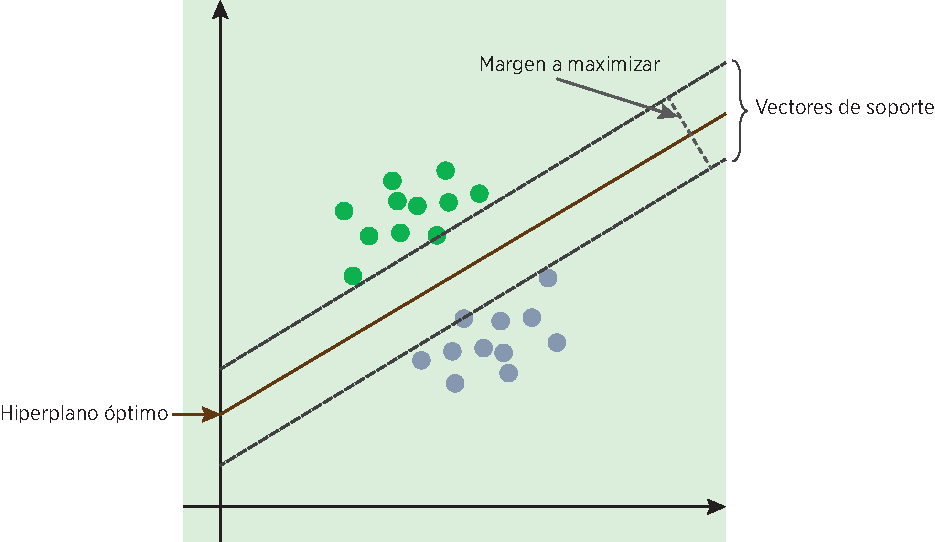
\includegraphics{imagenes/svm}
\par\end{centering}

\protect\caption{Identificación de vectores de soporte e hiperplano óptimo.\label{fig:Identificacion-de-vectores}}


\end{figure}



\section{Metodología}

La actividad consistió en realizar el conjunto de pasos descrito en el Algoritmo \ref{alg:algoritmo-svm} para realizar el entrenamiento y la clasificación utilizando las máquinas de soporte vectorial.
% \begin{algorithm} 
% \begin{algorithmic}[1] 
% \STATE Crear matriz Hessiana $H = Ytr_i,Ytr_j,K(Xtr_i,Xtr_j)$
% \STATE Encontrar $\alpha$, tal que 
% $\underset{\alpha}{max\left[\stackrel[i=1]{N}{\sum}\alpha_{i}-\frac{1}{2}\alpha^{T}H\alpha\right]} \text{sujeto a}~ 0\leq \alpha_{i}\leq{C} ~\forall i ~\text{y}\sum_{i=1}^{N}\alpha_{i}y_{i}=0$
% \STATE Determinar los vectores de soporte $\left\{x_{s},y_{s} \right\}$ que satisfacen la condición $ 0 < \alpha_{i} <  {C} $.
% \STATE Calcular el bias:
% $w_{0}=\frac{1}{N_s}\sum_{s\in S}\left\{ y_s - \sum_{m\in S}\alpha_m y_m K(x_m , x_s) \right\}$
% \STATE Dado un patrón $x'$, se clasificará según:
% $y' = \text{sign}\left\{ K(x_s , x')^{T} \alpha_s y_s + w_0 \right\}$
% \end{algorithmic} 
% \caption{Algoritmo para la clasificación con \emph{SVM}} 
% \label{alg:algoritmo-svm}
% \end{algorithm}


Se realizó la división de cada dataset en 70\% para entrenamiento y 30\% para prueba.
Asimismo, se preparó la secuencia de parámetros mostrada en la Tabla \ref{tbl:parametros} para la implementación de las funciones kernel lineal, polinomial y \emph{rbf} para cada uno de los cuatro datasets considerados en la asignación: \emph{BreastMG, BreastUS, Diabetes} y \emph{Heart}.